
\chapter*{Введение} \label{sec:intro}
\addcontentsline{toc}{chapter}{Введение}
%\pagestyle{plain}

В видо-временной системе всех нахско-дагестанских языков есть глагольные формы, подобные перфекту. Прототипический перфект указывает на совершенное в прошлом действие, которое имеет релевантность для момента речи --- свойство, получившее название \textsc{текущая релевантность} (current relevance) \citep[24--25]{comrie1985}. Пример (\ref{ex:just}) показывает употребление Перфекта со значением текущей релевантности в багвалинском языке нахско-дагестанской семьи.

\lb{ex:just}{\gll išːi-r haː-b-saʔatɬːi-r q'ani-r \textbf{q'ani-b-o} \textbf{ek'ʷa} \\
мы.{\Excl}-{\Erg} сей-{\N}-час-{\Erg} есть-{\Msd} есть-{\N}-{\Cvb} {\Aux}.{\Prs}\\
\trans `Мы {только} сейчас \textbf{покушали} (букв. еду съели).'  \\ \footnotesize{\citep[359]{tatevosov2007} \hfill багвалинский язык}}

Предложение в (\ref{ex:just}) не просто передает факт, что событие `поели' имело место в прошлом, но подчеркивает факт (в данном случае недавнего) завершения этого события и наличие у него имплицитных последствий. Предложение с Перфектом в (\ref{ex:just}) уместно, например, в контексте, описанном С.Г. Татевосовым, где говорящий Х говорит: <<Пусть твой брат приходит ко мне обедать>>, а говорящий Y ему отвечает: <<Вряд ли он пойдет.>> Высказывание в (\ref{ex:just}) представляет причину или объяснение того, почему брат говорящего Y вряд ли пойдет: они только что поели (импликация: брат еще сыт) (ibid.).\footnote{Для сравнения: общее прошедшее время (в случае багвалниского языка - Претерит) передавало бы просто факт, что кто-то поел, без импликаций для момента речи.}
\par В нахско-дагестанских языках такого рода формы часто приобретают дополнительное значение: говорящий сам не был свидетелем сообщаемого события. Ср. пример (\ref{ex:ali}), также из багвалинского языка.\label{p:context}

\lb{ex:ali}{\gll ʔali-r sĩː \textbf{k'ʷa-b-o} \textbf{ek'ʷa}\\
Али-{\Erg} медведь убивать-{\N}-{\Cvb} {\Aux}.{\Prs}\\
\trans `Али [, я слышал] \textbf{убил} медведя.'\\
`Али [, я вижу] \textbf{убил} медведя.' \\ \footnotesize{\citep[360]{tatevosov2007} \hfill багвалинский язык}}

В примере (\ref{ex:ali}), Перфект указывает на то, что говорящий узнал о том, что `Али убил медведя' каким-то косвенным образом: например, кто-то ему об этом рассказал --- \textsc{репортатив} (hearsay); или он видел какие-то очевидные последствия (например, он видел, как Али разделывал тушу медведя) и на основе этих косвенных свидетельств делает вывод, что событие имело место --- \textsc{инферентив} (inferential). Конкретная интерпретация определяется контекстом, и понятие \textsc{непрямой эвиденциальности} (indirect evidentiality) или более распространенный в русскоязычной лингвистике термин \textsc{косвенная засвидетельствованность} объединяют эти два значения. 

\par \textsc{\textbf{Эвиденциальность}} --- грамматическая категория, которая маркирует источник информации, лежащий в основе высказывания \citep[1]{aikhenvald2018}, например чужие слова или умозаключение в слуае примера (\ref{ex:ali}). В лингвистической типологии категория эвиденциальности является относительно молодым концептом.\footnote{Феномен грамматического маркирования источника информации впервые был отмечен давно, согласно \citep[125]{friedman2018} в \textsc{iv} веке до н.э. в санскритской грамматике Панини. Однако первое описание этого значения как грамматической категории обычно приписывают американскому лингвисту и этнографу Францу Боасу, который обнаружил эту категорию в языке квакиутль \citep[12]{aikhenvald2004}. Сам термин ввел Р.О. Якобсон (опираясь на материал болгарского языка и языка хопи) в статье \textit{Shifters, verbal categories and the Russian verb} \citep[41--58]{jakobson1957}.} Интерес к ней рос экспоненциально именно последние 20 лет, что доказывает актуальность настоящего исследования, посвящённого эвиденциальности как одному из значений перфектоподобных форм в языках нахско-дагестанской семьи.

\begin{figure}[H]
\centering
\caption{Количество публикаций по ключевому слову evidentiality}
\label{fig:evpubs}
\vspace{0.5cm}
\fbox{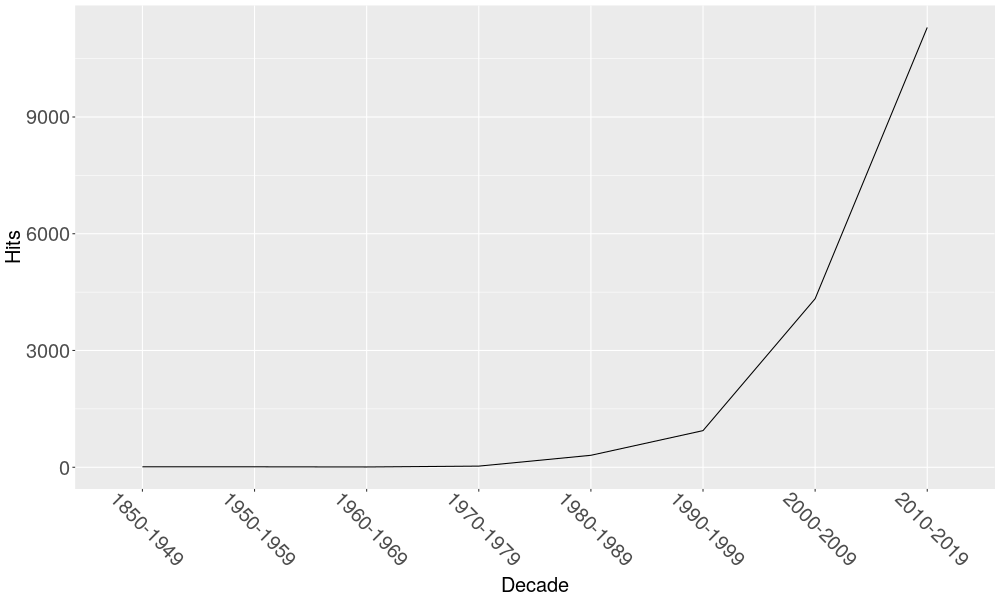
\includegraphics[scale=0.35]{images/evpubs.png}}
\end{figure}

Рисунок \ref{fig:evpubs} показывает число публикаций по ключевому слову \textbf{<<evidentiality>>} в поисковой системе академических текстов Google Scholar (по десятилетиям).\footnote{Поисковая система Google Scholar подбирает результаты по наличию ключевого слова, и упорядочивает их в поле результатов по релевантности, учитывая полный текст публикации, где она была опубликована, кем была написана, сколько раз и когда была процитирована, см. \href{https://en.wikipedia.org/wiki/Google_Scholar}{статью о поисковой системе в Википедии}. Результаты не отражают точную историю выхода публикаций по теме, во-первых, потому что эвиденциальность не всегда называлась эвиденциальностью и, во-вторых, потому что некоторые публикации алгоритмом не считаются релевантными. В наших поисковых результатах, например, основополагающая статья Р.О. Якобсона (см. предыдущую сноску) отсутствует в периоде 1950--1959, что возможно связано с тем, что эвиденциальность не является главной темой этой работы. Хотя термин \textsc{evidential} в этой публикации использовался впервые, он упоминается лишь кратко в рамках обсуждения типологии глагольных категорий. Стоит также напомнить что количество отражает только англоязычные публикации.} За период 1850--1949 вышло лишь 11 публикаций, и ни в одной из них не обсуждается именно лингвистическая эвиденциальность.\footnote{Помимо лингвистики, термин \textsc{эвиденициальность} употребляется в том числе в академических текстах по философии и психологии. Мы считаем не очень вероятным, что рост числа публикаций по теме эвиденциальности может быть связан с параллельным развитием данного понятия в этих дисциплинах, хотя следует признать, что мы не изучали содержание списков результатов для последних двадцати лет. Можно сказать тем не менее, что по крайней мере на первых страницах абсолютно доминируют лингвистические публикации, что указывает на то, что самые цитируемые работы по эвиденциальности на данный момент --- это работы по лингвистике.}
\par В период 1980--1989 количество публикаций начинает быстро увеличиваться (+307 по сравнению с предыдущими периодами), особенно после 1986-го года, когда вышел в свет широко цитируемый сборник \textit{Evidentiality: The linguistic encoding of epistemology} под редакцией Джоханны Николс и Уоллеса Чэйф \citep{chafenichols1986}. В 1999 г. Жильбер Лазар замечает: <<Evidentiality seems to be currently in fashion>> \citep[91]{lazard1999}, но это оказалось только началом. В период 1990--1999 выходит 941 публикация, а в 2000--2009 годах насчитывается уже 4.330 публикаций, причем рост наблюдается в основном после выхода в 2004-м году авторитетного типологического исследования А.Ю. Айхенвальд \textit{Evidentiality}, подготовленного на основе большого количества описаний языков \citep{aikhenvald2004}. На момент поискового запроса (в апреле 2019-го года) в период с 2010-го по 2019 год вышло 11.300 публикаций.
\par За это время накопилась богатая литература о категории эвиденциальности в отдельных языках. Выясняется, что у языков, распространенных на географически смежных территориях, встречаются похожие системы маркирования эвиденциальности, и категория в общем считается легко заимствуемой. Можно выделить по крайней мере пять разных <<эвиденциальных ареалов>> \citep[19--23]{plungian2010}. Территория нахско-дагестанских языков находится в центре одного из таких ареалов, охватывающего в том числе балканские, кавказские, финно-угорские, тибето-бирманские и тюркские языки. Тюркские языки многими исследователями считаются вероятными источниками распространении категории эвиденциальности в этом регионе \citep[265]{chirikba2003}, поскольку эта категория в той или иной степени присутствует во всех современных тюркских языках, и обладает доказанной древностью (подробнее об этом в разделах \ref{sec:pftyp} и \ref{sec:dagturk}). При этом, тюркские языки географически разбросаны почти по всему ареалу, включая Кавказ, и их носители могли находиться в контакте с носителями других языков. 
\par Эвиденциальные системы, характерные для данного ареала, иногда называют \textsc{малыми} \citep{aikhenvald2004}: они отличают незасвидетельствованные от засвидетельствованных событий.\footnote{По сравнению, в амазонских языках, например, отмечены до пяти разных маркированных источников, различая,  например, зрительное восприятия от аудиторного и других способов чувственного восприятия.} Основой этих систем часто являются перфектоподобные или <<перфектоидные>> формы со значением косвенной засвидетельствованности. Термин \textsc{перфектоид} используется В.А. Плунгяном для обозначения таких глагольных форм из выше описанного ареала, которые имеют некоторое сходство с прототипическими перфектами как находятся, например, в западноевропейских языках (ср. также пример (\ref{ex:just}) в начале этого введения), но которые при этом, помимо текущей релевантности, приобретают дополнительное эвиденциальное значение \citep[14--15]{plungian2016}. Поскольку термин \textsc{перфект} часто отождествляется с семантикой текущей релевантности, термин \textsc{перфектоид} нам кажется удобным способом описать предмет настоящего исследования, поскольку он одновременно подчеркивает и сходство, и различие с прототипическими перфектами.
\par Помимо ее особенного диахронического источника и частотности ее распеделения в определенном регионе, перфектоидная эвиденциальность особенна еще тем, что многие исследователи языков или языковых семей, принадлежащих вышеописанному ареалу, предпочитают вовсе не называть это явление <<эвиденциальностью>>, см. в том числе \citep{johanson2000}, \citep{friedman2000}, \citep{lazard1999}. Хотя предложенные альтернативные термины различаются, мнение этих авторов глобально заключается в том, что указание на источник информации не является \textit{главной функцией} этих форм. Несмотря на то, что перфектоиды часто используется в ситуациях, где говорящий сам не наблюдал события, категория эвиденциальности с их точки зрения не способна объяснить все употребления соответствующих форм (помимо текущей релевантности и косвенной засвидетельствованности). Формы могут употребляться, например, когда человек сам был свидетелем, но информация является новой или неожиданной --- \textsc{миративность} \citep[36]{delancey1997}, или считается говорящим менее достоверной --- \textsc{эпистемическая модальность} \citep[1--6]{boye2012}. Обе эти концептуальные категории встречаются как самостоятельные грамматические категории в языках мира, но часто они достаточно часто (хотя необязательно) сопровождают семантику косвенной засвидетельствованности.
\par В связи с этим, некоторые авторы пользуются более обобщенными концептами, такими как \textsc{медиатив} (фр. médiatif, англ. mediative) , ср. в том числе \citep{lazard1956} и \citep{lazard1999}, обозначая главным образом \textit{дистанцирование} говорящего от передаваемой им информации. В зависимости от контекста, причиной дистанции может быть отсутствие прямого доступа к событию (эвиденциальность) или неожиданность информации (миративность) \citep[95]{lazard1999}. Другие авторы различают несколько отдельных дополнительных значений, считая одно из них (чаще всего эвиденциальное) основным, а другие --- \textsc{расширением} собственно эвиденциальной семантики, то что называется extension в \citep{aikhenvald2004}. Предполагается, что эти дополнительные значения являются вторичными импликатурами, которые носители приписывают косвенной засвидетельствованности.
\par Судя по описаниям, конфигурации этой функциональной полисемии весьма своеобразны в отдельных языках. Балканские языки, например, считаются более <<модализированными>> \citep[354]{plungian2001}, т.е. главная функция перфектоидов в этих языках --- передача личного отношения говорящего к сообщаемой информации как более или менее достоверной (т.е. эпистемическая модальность). Как правило, оценка статуса разных значений относительно друг друга основана на впечатлениях отдельных исследователей, которые изучали употребление форм в одном языке разными методами: элицитацией, анализом письменных текстов и разговорной речи. Естественно, чтобы понимать, как функционируют в языке столь разносторонние формы, нужно рассматривать данные из самых разных типов дискурса с учетом ситуативного контекста. Проблема таких подходов для сопоставительного анализа заключается в том, что исходный языковой материал на основе которого сделаны выводы автора обычно недоступен или не полностью доступен исследователям-типологам, и в последствии мы вынуждены делать выводы на основе описаний и нескольких примеров, что не позволяет провести сопоставительного анализа собственно языкового материала. Работы об эвиденциальности в целом направлены скорее на изучение категории в отдельных языках. Сопоставительные исследования опираются на такие описания и в результате имеют обзорный характер. Сравниваются скорее описания признаков, чем собственно языковой материал.
\par В целях сравнения часто используется метод элицитации примеров или контекстов, которые в других языках оказались показательными. Известно, например, что формы косвенной засвидетельствованность плохо сочетаются с действующим субъектом первого лица, поскольку человек обычно является свидетелем собственных действий. В связи с этим, наблюдаются разные \textsc{эффекты первого лица}, в плане частотности употребления показателей косвенной засвидетелсьтвованности с субъектом первого лица, но и в плане интерпретации таких конструкций \citep{curnow2002}. Если показатель косвенной завсидетельствованности сочетается с субъектом первого лица, часто возникает интерпретация, что говорящий совершил действие \textit{неосознанно}, например, потому что он спал или был пьян. Считается, что если сочетание с первым лицом дает эффект неосознанности, то это хороший индикатор присутствия эвиденциального значения. Тем не менее, при работе с таким категориями как эвиденциальность, интерпретация которых сильно зависит от дискурсивного контекста, метод элицитации отдельных предложений имеет определенные недостатки. Ситуация элицитации может ощущаться носителем как неестественная, и соответственно и использование (глагольных) форм будет неестественное. Например, носитель может использовать более нейтральную форму вместо более уместной в предложенном контексте эвиденциальной формы потому, что ситуация элицитации не является естественной дискурсивной ситуацией, см. \citep[18]{aikhenvald2004}. Метод анализа корпусных данных также представляет определенные сложности: использование эвиденциальных форм в разных жанрах может регулироваться стилистическими правилами. Кроме того, эвиденциальности как грамматическая категория широко представлена в малых, бесписьменных языках, для которых большие корпуса недоступны, см. обсуждение разного рода данных в исследовании эвиденциальности в \citep{kittila2018}.
\par \textbf{Цель настоящего исследования} --- оценить статус компонента эвиденциальности в значении перфектоподобных форм в сопоставительной перспективе, и следовательно оценить статус этих форм в грамматике нахско-дагестанских языков. Кроме того, мы пытаемся оценить вероятность того, что этот признак появился в рассматриваемых языках под влиянием контакта с местными тюркскими языками. Для этого необходимо учитывать формальные свойства форм, их ареальное распространение и данные об истории языковых контактов. Эта цель подразумевает решение следующих \textbf{задач}:

\begin{itemize}
    \item \textbf{Инвентаризация и сравнительный анализ} формальных и семантических признаков нахско-дагестанских <<перфектоидов>> и их распределения по ветвям семьи и по территории Восточного Кавказа для выявления генеалогических или ареальных паттернов; сравнение релевантных признаков нахско-дагестанских форм с особенностями аналогичных форм в местных тюркских языках на общем фоне грамматики и выражения эвиденциальности в исследуемых языках.
    \item \textbf{Сравнительный анализ употребления перфектоидов,} что подразумевает разработку метода и меры сопоставления, поскольку имеющиеся подходы к анализу такого рода форм были направлены на описание эвиденциальности в разных языках, и результирующие данные часто трудно сопоставимы.
\end{itemize}

Для решения второй задачи мы предлагаем анализ употребления перфектоидов в нарративных цепочках. Известно, что прототипический перфект не может использоваться в цепочке клауз или предложений о последовательных событиях, и употребление перфектной формы в качестве нарративного времени считается признаком более продвинутой стадии ее грамматикализации, см. \citep{lindstedt2000}. Тем не менее, роль перфектоидов в повествованиях неоднозначна. Их употребление в определенных жанрах может подвергаться конвенционализации, при которой выбор форм диктуется скорее нарративными нормами чем источником информации говорящего. При этом, чередование перфектоида с основным прошедшим в текстах может служить как средство структурирования дискурса, помимо эвиденциальной функции. Существующие подходы к анализу эвиденциальных форм в нарративах рассматривают разные тексты целиком, описывая используемые формы и стараясь объяснить их распределение. Как многие другие работы об эвиденциальности вообще, они сосредоточены на изучение категории и ее особенностей в определенном языке, и не ставят себе целью сопоставительного анализа.
\par \textbf{Научная новизна} настоящего исследования состоит в попытке предложить метод сопоставительного анализа употребления в нарративных цепочках в разных жанрах повествования. При этом мы опираемся на формальные определения нарративной цепочки, используемые в \citep{labovwaletzky1967} и \citep{paducheva2010} для извлечения из данных по разным языками сопоставимых данных. \textbf{Теоретическая значимость} данной диссертации состоит в том, что она является первой попыткой систематического сравнения употребления эвиденциальных перфектоидов в нахско-дагестанских языках.

\par \textbf{Основные положения}, выносимые на защиту:

% Добавить что-то про типологию эвиденциальности

\begin{itemize}
    \item Перфектоподобные формы (перфектоиды) обнаруживаются во всех современных нахско-дагестанских языках, причем они могут выражать не только семантику косвенной засвидетельствованности, но и семантику текущей релевантности. При этом мы заметили тенденцию к развитию новых результативных конструкций.
    \item Показано, что выраженность действующего субъекта является фактором, различающим собственно результативное значение и значение результативного перфекта. Для нахско-дагестанских языков это является релевантным, поскольку результатив диахронически предшествует результативный перфект, и последнее может вовсе отсутствовать.
    \item Эвидециальное прочтение возникает в весьма разнородных условиях: %ДОПИСАТЬ.
    \item Значение косвенной засвидетельствованности как часть семантики перфектоида отсутствует в языках, находящихся на юге региона, где сильно влияние азербайджанский язык, в котором этот признак (в отличие от многих других современных тюркских языков) представлен слабо. Признак наоборот присутствует во многих языках северного и центрального Дагестана, где кумыкский язык (в котором признак представлен), исторически использовался как лингва франка; это указывает на то, что присутствие эвиденциальности в нахско-дагестанских языках может коррелировать с контактами с тюркскими языками, хотя наблюдаемая изоглосса требует дальнейшего изучения.
    \item Употребление перфектоидов в качестве нарративного заглазного времени оказывается важным диагностическим контекстом для определения наличия и возможно степени грамматикализации эвиденциального значения для нахско-дагестанских языков.
\end{itemize}

\textbf{Практическая значимость} работы состоит в дальнейшем применении используемых приемов анализа. Обзорная часть диссертации дает отправную точку для дальнейшего изучения исследуемых форм и их семантики в типологической перспективе. Во многих существующих описаниях не хватает детального описания условий, влияющих на интерпретацию формы, и примеров употребления многофункциональных форм, что затрудняет их интерпретацию в сравнении с якобы аналогичными формами в других языках. Разработанный в третьей главе метод для анализа естественных повествований позволяет сравнительный анализ разного рода текстового материала из разных языков по конкретным параметрам. Его применение при этом не ограничивается исследованием нахско-дагестанских языков.
\par \textbf{Основным материалом} исследования являются грамматики и специализированная литература об эвиденциальности и смежных явлениях в отдельных языках нахско-дагестанской семьи и в соседних тюркских языках. Сведения о формальных и функциональных аспектах эвиденциальности сопровождаются данными о социолингвистической ситуации на территории распространения нахско-дагестанских языков и о влиянии местных языков друг на друга. Материал третьей главы основан на проведенной автором полевой работе с разными диалектами андийского языка и анализа глоссированных текстах, опубликованных в грамматиках багвалинского и цахурского языков. Результаты работы прошли \textbf{апробацию} на разных международных конференциях, в том числе:

\begin{itemize}
    \item Tense, Aspect, Modality and Evidentiality (17-18 ноября 2016, Университет Дидеро, Париж) \\
    \textbf{Доклад:} Evidentiality and other usages of the perfect in Avar and Andi (Nakh-\\Daghestanian)
    \item Международная научная конференция <<Электронная письменность народов Российской Федерации: опыт, проблемы и перспективы>> (16--17 марта 2017, Сыктывкар) \\
    \textbf{Доклад:} Эвиденциальность и перфект в рутульском языке (на материале говора с. Кина)
    \item 50-я ежегодная конференция Европейского лингвистического общества \\ (SLE 2017) (10--13 сентября 2017, Университет Цюриха) \\
    \textbf{Доклад:} Evidentiality and the perfect in the Rikwani and Zilo dialects of Andi (East Caucasian)
    \item Четырнадцатая конференция по типологии и грамматике для молодых исследователей (23--24 ноября 2017, Санкт-Петербург) \\
    \textbf{Доклад:} Evidentiality in the Rikwani dialect of Andi
    \item 16-я конференция международной ассоциации прагматики (IPrA) (9--14 июня 2019, Политехнический Университет Гонконг) \\
    \textbf{Доклад:} Narrative use: a measurable feature of evidentiality as a meaning of the perfect
\end{itemize}

\par На момент аттестации вышли следующие публикации, из которых первая опубликована в сборнике, индексируемом в SCOPUS, вторая вышла в журнале из перечня ВАК, а третья вышла в журнале, индексируемом в SCOPUS Q1, и в Web of Science  Q4. % То есть журнал Web of Science Q4, а публикация нет?

\begin{enumerate}
    \item Verhees S. Chapter 12. The perfect in Avar and Andi: Cross-linguistic variation among two closely-related East Caucasian languages, in: Tense, Aspect, Modality and Evidentiality: Cross-linguistic perspectives. Amsterdam : John Benjamins Publishing Company, 2018. P. 261--280.
    \item Ферхеес С. К происхождению эвиденциальности в нахско-дагестанских языках: структурные и ареальные перспективы // Вестник Православного Свято-Тихоновского гуманитарного университета. Серия 3: Филология. 2018. № 57. С. 110--123.
    \item Verhees S. `General converbs in Andi'. \textit{Studies in Language}. 43:1 2019. P. 195--230.
\end{enumerate}

\textbf{Структура работы.} Диссертация состоит из введения, трех глав, заключения, списка литературы и нескольких приложений с собранными данными.\footnote{Данные также доступны в репозитории на Гитхабе: \url{https://github.com/sverhees/dissertation_evidentiality}} Во введении представлена общая характеристика работы. Первая глава посвящена эвиденциальности в типологической перспективе, с фокусом на перфектоидную эвиденциальность. Вторая глава представляет собой обзор эвиденциальности в нахско-дагестанских языках и включает ареальный анализ перфектоидов в нахско-дагестанских языках. Третья глава представляет анализ данных, полученных элицитацией у носителей разных диалектов андийского языка, и анализ нарративного материала из багвалинского и цахурского языков нахско-дагестанской семьи. Заключение суммирует основные результаты работы и обсуждает перспективы для дальнейшего исследования.
\par \textbf{Представление материала.} Примеры из языков приводятся в том виде, в каком они даны в оригинале, при необходимости добавлен русский перевод. В случае примеров из дагестанских языков транскрипция унифицирована (см. приложение  с таблицей соответствий). Если автор употреблял сокращения, которые нами не используются, они сохранены. Только глоссы, которые часто используются в нашей работе, унифицированы, например, конверб глоссируется нами как \textsc{cvb} (вместо используемого некоторыми авторами \textsc{conv}). В целом мы придерживаемся Лейпцигских правил глоссирования.\footnote{См. https://www.eva.mpg.de/lingua/resources/glossing-rules.php.} Нумерация рисунков и таблиц отдельная в каждой главе. Каждый пример сопровождается указанием на то, из какого он языка (иногда приводится более подробная информация о конкретном диалекте по схеме --- андийский: зиловский, т.е. андийский язык, зиловский диалект), и из какого источника он получен. Названия грамматических форм из конкретных языков обозначены заглавной буквой, а типологические или сравнительные концепты пишутся с маленькой буквы, как предложено в том числе в \citep{haspelmath2010}. Конкретные концепты при этом могут быть омонимами, ср. <<Типологически \textbf{перфект} ассоциируется с семантикой текущей релевантности>>, и <<В андийском языке \textbf{Перфект} имеет значение косвенной засвидетельствованности>>.
\par Для визуализации данных использовался язык программирования \textbf{R} и программный интерфейс \textbf{R Studio} \citep{r}. Непосредственно для лингвистических карт был использован пакет \textbf{lingtypology} \citep{lingtypology}, для работы с данными --- пакет  \textbf{tidyverse} \citep{tidyverse}, а для графиков --- \textbf{ggpubr} \citep{ggpubr}.

\section*{Благодарности}
Автор выражает благодарность научному руководителю М.А.~Даниэлю, за то, что он рискнул стать моим научным руководителем и в течение четырех лет неутомимо обсуждал со мной теоретические проблемы моей работы, Т.А.~Майсаку, за советы и обсуждения работы, и за то, что он доверил мне редактирование очерка ботлихского языка, Н.Р.~Добрушиной, которая помогала мне превращать свои мысли в публикуемые тексты, и обеспечила мне замечательное место работы в Лаборатории языковой конвергенции, моему любимому соавтору Г.А.~Морозу за помощь в программировании и дружбу, Кьяре Наккарато, которая все четыре года была рядом, а также рецензентам, которые тщательно и критично прочитали диссертацию, всем носителям андийского, ботлихского, аварского и других языков с которыми я работала, коллегам экспедиционерам, коллегам из лаборатории, коллегам кавказоведам и московской лингвистике в целом за то, что она такая интересная и дружелюбная. Говорят, что нужна целая деревня, чтобы воспитать одного ребенка. Чтобы воспитать меня как лингвиста их, как оказалось, нужно было несколько. Однако все недостатки работы (и их на момент публикации текста на сайте института, к сожалению, немало), естественно, мои.
